Interaction with computers can go far beyond keyboard typing and mouse pointing. Recent advances in computer vision technology can recognize hand gestures and body shape, as seen in Kinect games. With the new computer vision device such as Leap motion detector, it is possible to track the positions of each finger precisely. We propose a new method to control computers by interpret finger movements as commands or character input using finger tracking devices. 

Traditional character recognition technology is widely applied to such problems as converting scanned books to text and converting images of bank checks into valid payments. These problems can be divided into offline and online recognition. 

We introduce a new problem: the online recognition of characters in a stream of 3D points from fingers. Many OCR techniques utilize images of completed words, whereas this paper deals with interpreting the data while it is generated, specifically for the scenario of writing "in the air."  

With new innovations in computer vision, precise 3D finger data can be obtained at over 100 frames per second, so this paper also proposes a method of online character recognition, using a data-driven approach and a similarity search. We treat the input data from the computer vision device as a multivariate time series.

\marginpar{
\begin{figure}
  \begin{center}
  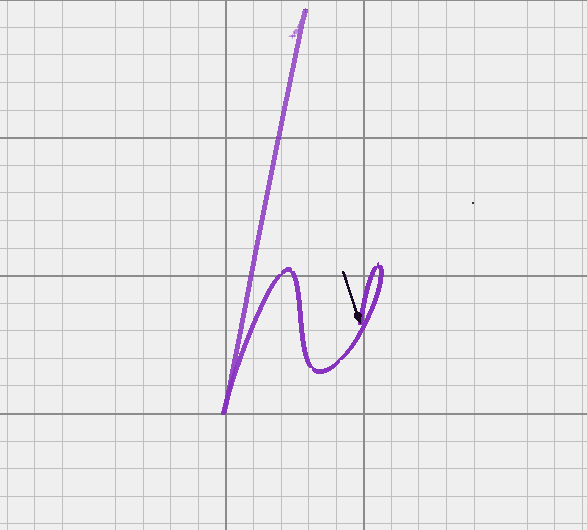
\includegraphics[width=1.75in]{images/he-2d-white-cropped.PNG}
  \caption{A 2D view of LEAP Motion data}
  \label{fig:teaser}
  \end{center}  
\end{figure}
}
The task of identifying characters in a time series requires data to test and train on. Therefore, a new dataset needs to be created, partitioned into multiple candidate time series, specifically the characters in the alphabet, and multiple testing time series, which are words to be recognized. To construct this dataset, the LEAP Motion, a commercial computer vision device, is used to record and store data. The experiment will consist of collecting the same data from 100 people to account for differences in handwriting.\\
The proposed approach to identify characters in these time series uses the dynamic time warping (DTW) algorithm. A series of recent optimizations make a DTW similarity search feasible in real time. This paper benchmarks the performance of such a similarity search with the given application of handwriting recognition.\\
